%TODO make paragraph

\section{Initial Concept}

\silvia{this section is too difficult to understand, need a complete rewrite}

\silvia{i think this should be a separate section. give it a name (seed concept? seed design?) - just "seed" is not enough. There was also some study done prior to this design (interviews, study, observation).
briefly report this in 2.1. Then you can present the first design itself (fig 2.1)}

Restricting the use of data to one user is undesirable, therefore good data management has to be applied to enable re-use.
\silvia{explain where the initial idea came from (maybe this is the link with the previous part?)}
The initial idea in this project was to develop a data management system with data-centric functions, \eg{} request, upload, download, search, for .....
These are represented in figure \ref{fig:research-workflow} with the blocks `request' and `data'.
With these functions a big part of the research workflow would be supported.


\silvia{
the txt below was at the caption, but i think it should not. captions are used to explain the figure - nothing else. generic stuff goes to the text body:
External services such as .. are provided ?? and outside of the scope of this paper.
Two direct users and several external users are planned each with their specific set of functions.
		Data listed is either available at initialisation of the system or is generated during execution.
}
		
\begin{figure}[t]
	\centering
	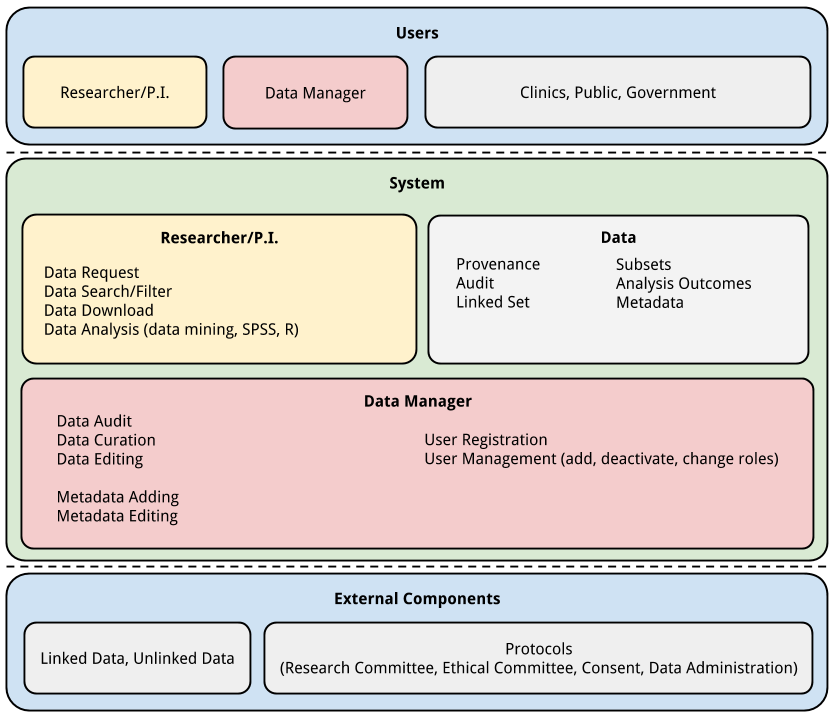
\includegraphics[width=1.0\linewidth]{images/brainstorm-before}
	\caption{
		Initial concept for the \ivfsystem{}, encompassing data and user management. 
		The system offers different sets of functions for three user roles (a,b,c) indicated by colours. 
		External services provide data according to regulations.
	}
	\label{fig:brainstorm-before}
\end{figure}

Figure \ref{fig:brainstorm-before} describes the full view of the seed. The function groups are expanded into: users, external services, data, and functions.
The external services provide ...
They influence the system but are outside of the scope of this paper.
This means that data and protocols (necessary for lawful execution of the system) 
are already provide by these external systems, and ???.
From the provided data, unlinked data is \project{} data split into clinics and PRN, where linked data are the matched rows from both.
Projected direct users are researchers and data managers.
Furthermore, external parties (clinics, public, government) might be interested in statistics of the system and its data, \eg{} aggregated and anonymised analysis outcomes.

Functions for each of the user roles encompass data management and user management.
Data functions meaning mutations of the raw \project{} data, where metadata is metadata of this raw data. \silvia{need to explain in intro what is data, metadata in general and in the context of this project}
The data block refers to data being stored in the system at initialisation and during execution.
The linked set (\ie{} raw data) is an initialisation input of the system.
Other items are generated during execution, \eg{} subsets are created after a data request is granted which also results in provenance data, etc.